\chapter{대칭성과 보존 법칙}

\lectureoverview{정지 작용과 오일러--라그랑주 방정식은 고전역학의 핵심 절반이고, 해밀턴 형식은 나머지 절반이다. 여기서는 첫 번째 절반을 충분히 전개하여 하나의 심오한 규칙을 드러내겠다. 라그랑지안의 모든 연속 대칭은 보존량을 만들어 낸다. 병진과 회전에서 이 규칙을 찾아보고, 일반적인 무한소 변환에 대해 증명한 다음, 이 논증이 적용되는 경우와 적용되지 않는 경우를 자세히 살펴보겠다.}

\section{물리를 설명하는 데 필요한 최소한의 수학}

칠판에 이미 적힌 식들은 슈뢰딩거 방정식과 조금 닮아 보일지 모르지만, 오늘 다룰 주제는 그것이 아니다. 주제는 대칭성과 보존이다. 방정식 없이 이 둘의 관계를 제대로 설명할 방법은 없다. 방정식 자체는 기초적이다. 중요한 것은 구조가 눈에 드러나도록 식들을 배열하는 일이다. 결과의 이름은 Scientific American에서 따올지 모르지만, 여기서는 물리학자가 유도하듯 그 결과를 이끌어 내는 데 필요한 최소한의 수학을 다루고자 한다.

작은 매개변수 \(\epsilon\)를 도입하자. \(\epsilon\)에 비례하는 항은 남기고 \(O(\epsilon^2)\)은 버린다. 이는 극한 논증을 줄여 쓴 것이지, 영이 아닌 실수의 제곱이 문자 그대로 영이라는 주장은 아니다. 보통 함수 \(f(x,y)\)에 대해서는
\begin{equation}
  \delta f
  =\frac{\partial f}{\partial x}\,\delta x
   +\frac{\partial f}{\partial y}\,\delta y
   +O(\epsilon^2),
  \label{eq:first-variation-f}
\end{equation}
여기서 \(\delta x\)와 \(\delta y\)는 모두 \(\epsilon\)에 비례한다. 기호 \(\delta f\)는 \(f\)의 변화를 뜻하며, \(\delta\)라는 수와 \(f\)의 곱을 뜻하지 않는다. 정지점에서는 다음을 만족한다.
\begin{equation}
  \delta f=0
  \qquad\hbox{to first order.}
  \label{eq:stationary-f}
\end{equation}

역학적 경로 \(q_i(t)\)에 대응하는 양은 작용이다.
\begin{equation}
  S[q]=\int_{t_1}^{t_2}L(q,\dot q,t)\,dt.
  \label{eq:action-l4}
\end{equation}
양 끝점을 고정한 채 경로를 변분하면
\begin{equation}
  \delta S
  =\int_{t_1}^{t_2}dt\,
   \sum_i\left(
     \frac{\partial L}{\partial q_i}\,\delta q_i
     +\frac{\partial L}{\partial\dot q_i}\,\delta\dot q_i
   \right).
  \label{eq:action-variation-l4}
\end{equation}
두 항이 나타나는 이유는 경로를 바꾸면 위치와 속도가 모두 바뀌기 때문이다. 부분적분과
\(\delta q_i(t_1)=\delta q_i(t_2)=0\)를 함께 이용하면 \(\delta S=0\)는 다음과 같이 된다.
\begin{equation}
  \frac{d}{dt}\left(\frac{\partial L}{\partial\dot q_i}\right)
  -\frac{\partial L}{\partial q_i}=0.
  \label{eq:el-l4}
\end{equation}

\begin{figure}[htbp]
  \centering
  \includegraphics[width=0.76\textwidth]{lecture_04_figure_05.png}
  \caption{대칭성과 보존을 논의할 출발점으로 다시 살펴보는 오일러--라그랑주 방정식.}
  \lectureframe{00:09:00}
\end{figure}

정확한 표현은 \emph{정지 작용}이지, 반드시 최소 작용인 것은 아니다. 이 차이는 끝부분에서 다시 다루겠다.

\section{일반화 좌표와 켤레 운동량}

일반적인 역학을 표현하기에는 데카르트 좌표만으로는 부족하다. 좌표는 입자의 위치, 각도, 집단 변수 또는 장의 진폭일 수 있으므로 이를 \(q_i\)라 부른다. 라그랑지안은 동역학을 압축해 기술한다. 표준 모형을 아주 압축된 표기 없이 전부 적으면 대략 한 페이지를 차지한다. 장의 각 성분마다 운동 방정식을 따로 적는다면 훨씬 더 많은 지면이 필요할 것이다. 하나의 함수 \(L\)가 그 모든 내용을 담는다.

\(q_i\)에 켤레인 운동량은
\begin{equation}
  p_i=\frac{\partial L}{\partial\dot q_i}.
  \label{eq:canonical-momentum-l4}
\end{equation}
이 때문에 일반화 좌표를 전통적으로 \(q\)라 부르고, 이에 대응하는 운동량은 \(p\)라 부른다. 따라서 \(p\)와 \(q\)를 얻게 된다. 이 표기법으로 식 ~\eqref{eq:el-l4}는 다음과 같다.
\begin{equation}
  \dot p_i=\frac{\partial L}{\partial q_i}.
  \label{eq:momentum-el-l4}
\end{equation}

익숙한 1차원 입자의 경우,
\begin{equation}
  L=\frac{m\dot x^2}{2}-V(x),
  \qquad
  \frac{\partial L}{\partial\dot x}=m\dot x,
  \label{eq:particle-momentum-l4}
\end{equation}
따라서 켤레 운동량은 보통의 운동량이다.

\begin{figure}[htbp]
  \centering
  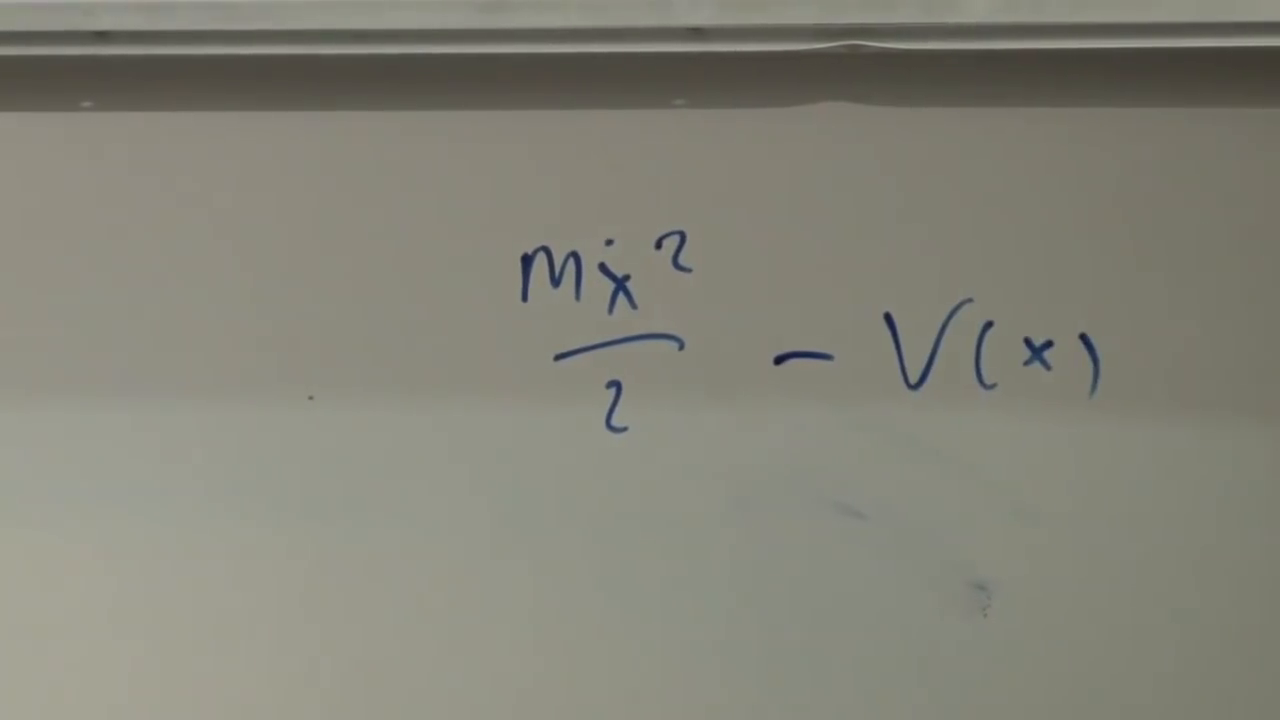
\includegraphics[width=0.72\textwidth]{lecture_04_figure_02.png}
  \caption{켤레 운동량을 \(m\dot x\)와 동일시할 때 사용하는 운동에너지에서 퍼텐셜 에너지를 뺀 라그랑지안.}
  \lectureframe{00:14:48}
\end{figure}

\(q_i\)가 \(L\)에 나타나지 않으면 \(\dot p_i=0\)이다. 이는 보존 법칙을 얻는 익숙한 순환좌표 방법이다. 실제 관계는 더 일반적이며, 이를 증명하기에 앞서 예시를 통해 알아보면 유익하다.

\section{설명에 앞서 살펴보는 보존 법칙}

\subsection{두 좌표와 두 좌표의 차이에만 의존하는 퍼텐셜}

두 질량을 모두 1로 두고 다음과 같이 하자.
\begin{equation}
  L=\frac{\dot q_1^{\,2}+\dot q_2^{\,2}}{2}-V(q_1-q_2).
  \label{eq:separation-lagrangian}
\end{equation}
두 입자가 직선 위에 있다고 생각해도 좋다. 두 입자의 상호작용은 서로의 간격에만 의존한다.

\begin{figure}[htbp]
  \centering
  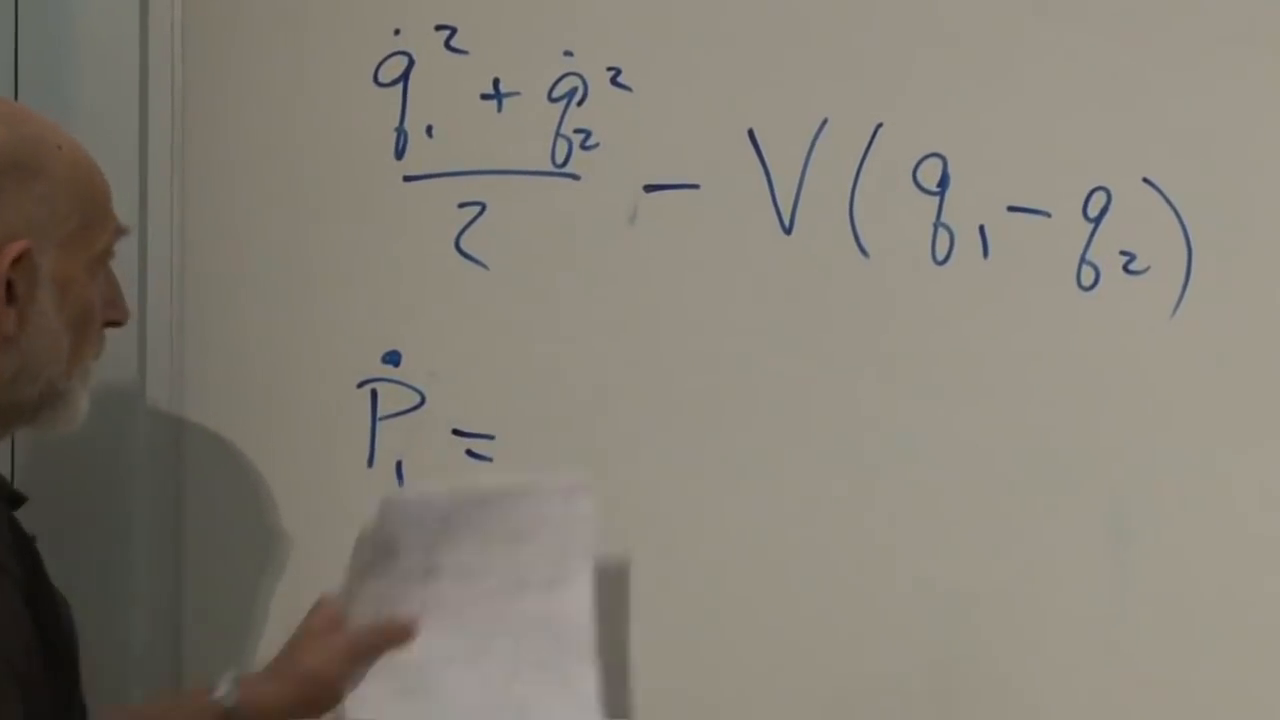
\includegraphics[width=0.78\textwidth]{lecture_04_figure_03.png}
  \caption{두 좌표에 대한 라그랑지안과 첫 번째 운동량 방정식의 시작 부분.}
  \lectureframe{00:18:56}
\end{figure}

\(V\)의 인수에 대한 미분을 \(V'\)로 쓰면,
\begin{align}
  \dot p_1&=-V'(q_1-q_2),
  \notag\\
  \dot p_2&=+V'(q_1-q_2).
  \label{eq:separation-momentum-equations}
\end{align}
\(q_2\)를 증가시키면 \(q_1-q_2\)가 감소하므로 두 번째 식의 부호는 반대가 된다.

\begin{classroomqa}
  \audiencequestion{첫 번째 운동량 방정식에 \(V'\)가 들어가야 하나요? 마이너스 부호는 어디서 나오나요?
  \lecturetimestamp{00:20:52--00:21:35}}
  \lecturerresponse{오일러--라그랑주 방정식은 라그랑지안이 0이라는 뜻이 아니라
  \(\dot p_1=\partial L/\partial q_1\)라고 말합니다.
  \(L=T-V\)이므로 \(q_1\)에 대해 미분하면
  \(-V'\)가 됩니다. \(q_2\)에 대해 미분하면 \(q_1-q_2\)에서 마이너스 부호가 하나 더 생기므로, 두 번째 방정식에는 \(+V'\)가 들어갑니다.}
\end{classroomqa}

\begin{figure}[htbp]
  \centering
  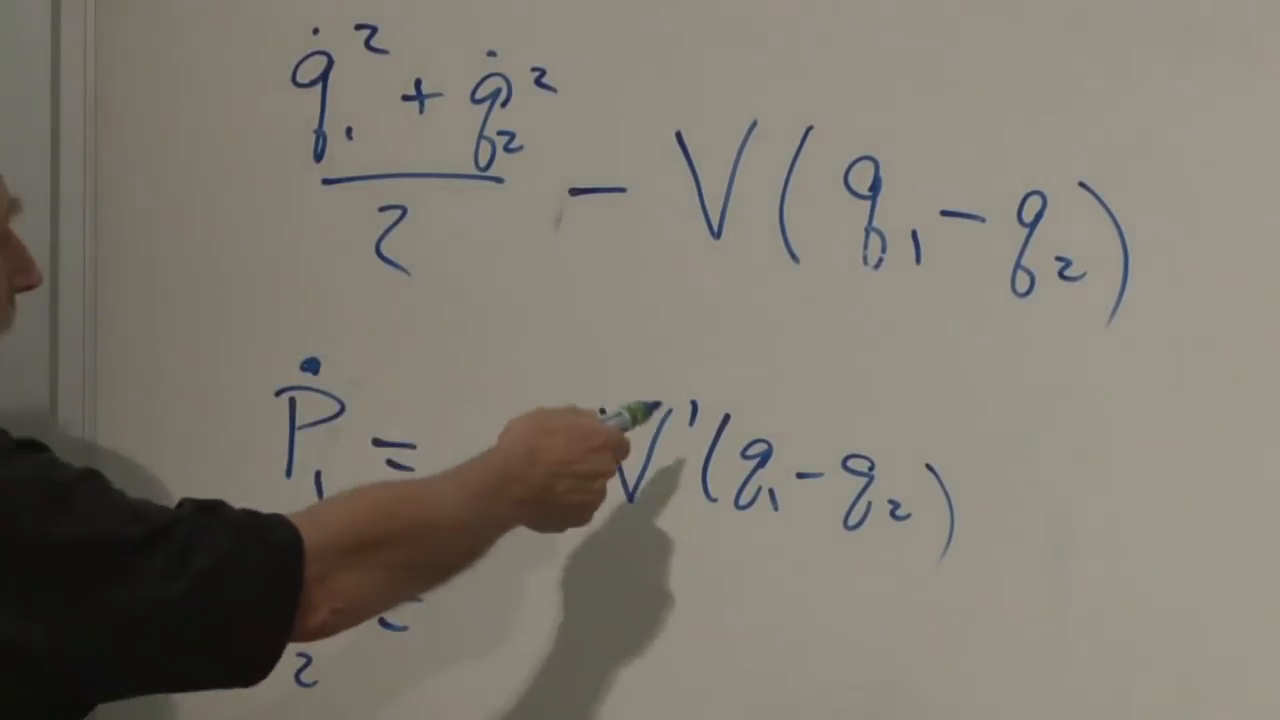
\includegraphics[width=0.78\textwidth]{lecture_04_figure_04.png}
  \caption{부호에 민감한 \(p_1\) 방정식의 미분. \(p_2\) 방정식에는 반대 부호가 붙는다.}
  \lectureframe{00:20:41}
\end{figure}

식 ~\eqref{eq:separation-momentum-equations}를 더하면
\begin{equation}
  \frac{d}{dt}(p_1+p_2)=0.
  \label{eq:total-p-conserved}
\end{equation}
보존량을 찾았지만, 그것이 왜 존재하는지는 아직 설명하지 않았다.

\subsection{덜 자명한 선형 결합}

이제
\begin{equation}
  L=\frac{\dot q_1^{\,2}+\dot q_2^{\,2}}{2}
    -V(Aq_1+Bq_2),
  \label{eq:ab-lagrangian}
\end{equation}
라 하자. 여기서 \(A\)와 \(B\)는 상수이다. 그러면
\begin{align}
  \dot p_1&=-A\,V'(Aq_1+Bq_2),
  \notag\\
  \dot p_2&=-B\,V'(Aq_1+Bq_2).
  \label{eq:ab-momentum-equations}
\end{align}
첫 번째 방정식에 \(B\)를 곱하고, 두 번째 방정식에 \(A\)를 곱한 뒤 두 식을 빼면 힘 항이 소거된다.
\begin{equation}
  \frac{d}{dt}(Bp_1-Ap_2)=0.
  \label{eq:ab-conserved}
\end{equation}

\begin{figure}[htbp]
  \centering
  \includegraphics[width=0.78\textwidth]{lecture_04_figure_06.png}
  \caption{가중 운동량 방정식에서 \(Bp_1-Ap_2\)의 힘 항들이 서로 상쇄된다.}
  \lectureframe{00:24:20}
\end{figure}

\begin{classroomqa}
  \audiencequestion{\(A\)와 \(B\) 같은 상수는 물리적으로 어디에서 올 수 있을까요?
  \lecturetimestamp{00:25:09--00:30:15}}
  \lecturerresponse{질량이 \(m\)와 \(M\)인 두 입자를 생각해 봅시다.
  \[
    L=\frac{m\dot X^2}{2}+\frac{M\dot Y^2}{2}-V(X-Y).
  \]
  \(Q_1=\sqrt m\,X\)와 \(Q_2=\sqrt M\,Y\)로 재척도화합시다. 운동에너지 항은 \((\dot Q_1^2+\dot Q_2^2)/2\)가 되고, 퍼텐셜은 \(Q_1/\sqrt m-Q_2/\sqrt M\)에 의존합니다. 따라서 질량이 서로 다르면 선형 결합의 계수에 자연스럽게 질량 인자가 들어갑니다. \(Q_2\)를 \(-Q_2\)로 바꾸면 제곱된 운동에너지 항은 그대로인 채 식에 표시된 마이너스 부호가 플러스 부호로 바뀝니다.}
\end{classroomqa}

\begin{figure}[htbp]
  \centering
  \includegraphics[width=0.82\textwidth]{lecture_04_figure_07.png}
  \caption{질량 가중 좌표는 운동에너지를 간단하게 만드는 대신 질량 인자를 퍼텐셜로 옮긴다.}
  \lectureframe{00:28:40}
\end{figure}

\begin{classroomqa}
  \audiencequestion{이로써 순환좌표가 없어도 보존량이 존재할 수 있음을 보인 건가요?
  \lecturetimestamp{00:31:13--00:31:58}}
  \lecturerresponse{현재 적힌 변수에는 \emph{명백한} 순환좌표가 없습니다. 변수 변환을 하면 순환좌표가 드러날 수 있지만, 그것을 찾아다니는 관점은 여기서 유용하지 않습니다. 대칭성 논증은 보존되는 결합을 직접 찾아낼 것입니다.}
\end{classroomqa}

\section{대칭의 의미}

\subsection{병진}

질량이 단위 질량인 자유 입자에서 시작하자.
\begin{equation}
  L=\frac{\dot q^2}{2}.
  \label{eq:free-unit-l4}
\end{equation}
그 운동 이력의 모든 점을 동일한 상수만큼 평행이동시키자.
\begin{equation}
  q'(t)=q(t)+\epsilon.
  \label{eq:free-translation}
\end{equation}
\(\epsilon\)는 시간에 무관하므로 \(\dot q'=\dot q\)이고, 따라서 \(\delta L=0\)이다. 이 변환은 병진 대칭이다.

서로 동등한 관점이 두 가지 있다. 수동적 관점에서는 물체를 그대로 둔 채 좌표 원점만 옮긴다. 능동적 관점에서는 좌표축을 고정하고 물체를 움직인다. 능동적 표현이 덜 혼란스럽다. 물리적 배치를 움직였을 때 \(L\)가 달라지는지 묻는 것이다.

식 ~\eqref{eq:separation-lagrangian}에 대해 두 좌표를 모두 병진시키자.
\begin{equation}
  \delta q_1=\epsilon,
  \qquad
  \delta q_2=\epsilon.
  \label{eq:common-translation}
\end{equation}
속도는 변하지 않으며 \(q_1-q_2\)도 변하지 않는다.

\begin{figure}[htbp]
  \centering
  \includegraphics[width=0.78\textwidth]{lecture_04_figure_08.png}
  \caption{두 좌표를 함께 병진시키면 두 좌표 사이의 간격은 변하지 않는다.}
  \lectureframe{00:35:30}
\end{figure}

식 ~\eqref{eq:ab-lagrangian}에 대해서는 덜 자명한 변환을 사용하자.
\begin{equation}
  \delta q_1=B\epsilon,
  \qquad
  \delta q_2=-A\epsilon.
  \label{eq:ab-transformation}
\end{equation}
이번에도 속도는 변하지 않으며,
\begin{equation}
  \delta(Aq_1+Bq_2)=AB\epsilon-BA\epsilon=0.
  \label{eq:ab-invariant-argument}
\end{equation}
따라서 이 변환은 대칭이다.

\begin{figure}[htbp]
  \centering
  \includegraphics[width=0.80\textwidth]{lecture_04_figure_09.png}
  \caption{를 보존하는 비대칭 병진.\(Aq_1+Bq_2\)}
  \lectureframe{00:40:20}
\end{figure}

\begin{classroomqa}
  \audiencequestion{이 계수들은 질량을 나타내며, 따라서 보존량은 보통의 질량중심 운동량이 되나요?
  \lecturetimestamp{00:42:25--00:42:45}}
  \lecturerresponse{그렇습니다. 질량 가중 변수에서는 대칭성과 보존되는 결합이 비대칭적으로 보입니다. 다시 \(X\)와 \(Y\)로 변환하면 보통의 동시 병진과 전체 운동량을 얻습니다.}
\end{classroomqa}

\subsection{회전}

평면에서 입자 하나를 생각하자.
\begin{equation}
  L=\frac{m}{2}(\dot x^2+\dot y^2)-V(x^2+y^2).
  \label{eq:central-lagrangian-l4}
\end{equation}
이는 중심 퍼텐셜이다. 서로 회전된 두 고정 좌표계를 비교하자. 좌표축은 시간에 따라 회전하지 않는다. 일관된 방향 규약을 택하면
\begin{align}
  x'&=x\cos\theta+y\sin\theta,
  \notag\\
  y'&=-x\sin\theta+y\cos\theta.
  \label{eq:finite-rotation-l4}
\end{align}

\begin{figure}[htbp]
  \centering
  \includegraphics[width=0.82\textwidth]{lecture_04_figure_10.png}
  \caption{중심 퍼텐셜을 가진 라그랑지안과 회전으로 서로 관계된 두 고정 데카르트 좌표계.}
  \lectureframe{00:45:40}
\end{figure}

\(\theta=\epsilon\)로 두고 1차 항까지만 남기자.
\begin{equation}
  \cos\epsilon=1+O(\epsilon^2),
  \qquad
  \sin\epsilon=\epsilon+O(\epsilon^3).
  \label{eq:small-angle-l4}
\end{equation}
무한소 회전은 다음과 같다.
\begin{align}
  \delta x&=y\epsilon,
  &\delta y&=-x\epsilon,
  \notag\\
  \delta\dot x&=\dot y\epsilon,
  &\delta\dot y&=-\dot x\epsilon.
  \label{eq:infinitesimal-rotation-l4}
\end{align}

\begin{figure}[htbp]
  \centering
  \includegraphics[width=0.82\textwidth]{lecture_04_figure_11.png}
  \caption{좌표와 속도의 무한소 회전.}
  \lectureframe{00:49:50}
\end{figure}

병진과 달리 \(x\)의 변화량은 \(y\)에 따라 달라지고, \(y\)의 변화량은 \(x\)에 따라 달라진다. 그럼에도
\begin{align}
  \delta(x^2+y^2)
  &=2x\,\delta x+2y\,\delta y=0,
  \notag\\
  \delta(\dot x^2+\dot y^2)
  &=2\dot x\,\delta\dot x+2\dot y\,\delta\dot y=0.
  \label{eq:rotation-invariants-l4}
\end{align}
퍼텐셜 항과 운동에너지 항은 모두 불변이다.

\begin{figure}[htbp]
  \centering
  \includegraphics[width=0.76\textwidth]{lecture_04_figure_12.png}
  \caption{제곱 반지름이 회전에 불변임을 보이는 1차 항의 상쇄.}
  \lectureframe{00:53:20}
\end{figure}

\section{일반적인 보존 정리}

병진과 회전의 예에는 공통된 형식이 있다. 연속적인 무한소 변환을 다음과 같이 두자.
\begin{equation}
  \delta q_i=\epsilon f_i(q),
  \qquad
  \delta\dot q_i=\frac{d}{dt}\delta q_i,
  \label{eq:general-infinitesimal-symmetry}
\end{equation}
여기서 \(\epsilon\)는 시간에 무관하며, \(f_i\)는 모든 좌표에 의존할 수 있다.

\begin{figure}[htbp]
  \centering
  \includegraphics[width=0.78\textwidth]{lecture_04_figure_13.png}
  \caption{일반적인 무한소 변위장 \(\delta q_i=\epsilon f_i(q)\)}
  \lectureframe{00:56:00}
\end{figure}

라그랑지안의 1차 변분은 다음과 같다.
\begin{equation}
  \delta L
  =\sum_i\left(
    \frac{\partial L}{\partial q_i}\delta q_i
    +\frac{\partial L}{\partial\dot q_i}\delta\dot q_i
  \right).
  \label{eq:delta-l-general}
\end{equation}

\begin{figure}[htbp]
  \centering
  \includegraphics[width=0.84\textwidth]{lecture_04_figure_14.png}
  \caption{\(\delta L\)에 기여하는 두 항: 좌표의 변분과 속도의 변분.}
  \lectureframe{01:02:30}
\end{figure}

이제 물리적 경로에 한정하면 오일러--라그랑주 방정식이 성립한다. 다음을 이용하면
\begin{equation}
  \frac{\partial L}{\partial\dot q_i}=p_i,
  \qquad
  \frac{\partial L}{\partial q_i}=\dot p_i,
  \label{eq:el-substitution-l4}
\end{equation}
다음 결과를 얻는다.
\begin{align}
  \delta L
  &=\sum_i\left(\dot p_i\,\delta q_i
                +p_i\,\delta\dot q_i\right)
  \notag\\
  &=\frac{d}{dt}\sum_i p_i\delta q_i
  =\epsilon\frac{d}{dt}\sum_i p_i f_i(q).
  \label{eq:noether-derivation-l4}
\end{align}
핵심 단계는 곱의 미분 법칙뿐이다.

변환이 대칭이면 \(\delta L=0\)이다. \(\epsilon\)는 임의의 상수 인자이므로
\begin{equation}
  \boxed{
  \frac{d\mathcal Q}{dt}=0,
  \qquad
  \mathcal Q=\sum_i p_i f_i(q)}
  .
  \label{eq:noether-charge-l4}
\end{equation}
이는 정확한 시간 독립 점 대칭에 대한 뇌터 정리의 고전역학적 핵심이다.

\begin{figure}[htbp]
  \centering
  \includegraphics[width=0.84\textwidth]{lecture_04_figure_15.png}
  \caption{곱의 미분 법칙을 이용해 \(L\)의 불변성으로부터 보존량을 얻는 단계.}
  \lectureframe{01:05:00}
\end{figure}

\begin{classroomqa}
  \audiencequestion{식 \(f_i(q)\)에서 \(q\)에 또 다른 첨자가 붙나요?
  \lecturetimestamp{01:06:57--01:07:31}}
  \lecturerresponse{첨자가 없는 \(q\)는 전체 집합 \((q_1,q_2,\ldots)\)를 뜻합니다. 각 성분 \(f_i\)는 그 좌표 전부에 의존할 수 있습니다. 예를 들어 회전의 경우 \(f_x=y\)이고 \(f_y=-x\)입니다.}
\end{classroomqa}

이제 예시들이 우연이 아님을 알 수 있다. 공통 병진에서는 \(f_1=f_2=1\)이므로
\begin{equation}
  \mathcal Q=p_1+p_2.
  \label{eq:noether-common-p}
\end{equation}
비대칭 병진에서는 \(f_1=B\), \(f_2=-A\)이므로
\begin{equation}
  \mathcal Q=Bp_1-Ap_2.
  \label{eq:noether-ab-p}
\end{equation}
회전에서는 \(f_x=y\)와 \(f_y=-x\)이므로
\begin{equation}
  \mathcal Q=p_xy-p_yx.
  \label{eq:rotation-charge-sign}
\end{equation}
방향 규약에 따른 부호 차이를 제외하면 이는 각운동량이다.
\begin{equation}
  J=xp_y-yp_x.
  \label{eq:angular-momentum-l4}
\end{equation}

\begin{figure}[htbp]
  \centering
  \includegraphics[width=0.82\textwidth]{lecture_04_figure_16.png}
  \caption{회전에 대한 뇌터 전하. 방향 규약에 따라 부호가 달라질 수 있지만 평면 각운동량과 같다.}
  \lectureframe{01:11:00}
\end{figure}

상호작용하는 입자가 여러 개라면 모든 입자를 함께 회전시킨다. 이때 불변성으로 보존되는 것은 각 입자의 각운동량이 따로가 아니라 각운동량의 합이다.

\section{정리의 가정에 관한 질문}

\begin{classroomqa}
  \audiencequestion{좌표축 집합을 회전시키면 \(\delta L\)에 명시적인 시간 의존성이 생기나요?
  \lecturetimestamp{01:12:57--01:13:57}}
  \lecturerresponse{그렇습니다. 방금 증명에서는 시간에 무관한 대칭 매개변수, 즉 고정된 병진이나 고정된 회전을 가정합니다. 매개변수가 시간에 의존하는 변환에는 추가 항이 생기므로 더 일반적인 처리가 필요합니다.}
\end{classroomqa}

\begin{classroomqa}
  \audiencequestion{칠판의 공식에 쓰인 대문자 \(Q\)가 변환 자체를 뜻하나요?
  \lecturetimestamp{01:14:02--01:15:58}}
  \lecturerresponse{아닙니다. 이 표기법은 안타깝게도 좌표 \(q_i\)와 겹칩니다. 변환은 \(\delta q_i=\epsilon f_i(q)\)이고, 그 결과 얻는 보존량은 \(\mathcal Q=\sum_i p_i f_i\)입니다. 계수 \(f_i\)는 대칭 변환 아래에서 \(i\)번째 좌표가 어떻게 움직이는지를 나타냅니다.}
\end{classroomqa}

에너지 보존도 대칭에서 비롯되지만, 다른 종류의 대칭이다. 시간에 대한 병진, 즉 시간의 원점을 어디에 두어도 물리가 달라지지 않는 성질이다. 이 경우와 해밀턴 형식은 뒤에서 다루겠다.

\begin{classroomqa}
  \audiencequestion{실제 운동을 변하는 좌표계에 흡수하여 역학을 좌표 변환만으로 설명할 수 있나요?
  \lecturetimestamp{01:17:43--01:20:01}}
  \lecturerresponse{특정한 운동을 따라가는 좌표를 선택할 수는 있지만, 그러면 그 변환은 초기 상태와 궤적에 의존합니다. 여기서 사용하는 대칭 변환은 계가 어떤 해를 따르는지와 무관하게 정해집니다. 운동 자체는 좌표와 운동량을 합친 공간에서 표현하는 편이 더 자연스럽습니다.}
\end{classroomqa}

\section{위상 공간에서의 조화 진동자}

질량과 용수철 상수를 각각 하나로 두면,
\begin{equation}
  L=\frac{\dot q^2}{2}-\frac{q^2}{2}.
  \label{eq:oscillator-l4}
\end{equation}
정준 운동량과 운동 방정식으로부터 다음을 얻는다.
\begin{equation}
  p=\dot q,
  \qquad
  \dot p=-q,
  \label{eq:oscillator-first-order-l4}
\end{equation}
또는
\begin{equation}
  \dot q=p,
  \qquad
  \dot p=-q.
  \label{eq:oscillator-phase-flow}
\end{equation}
이 방정식들은 \(q\)-\(p\) 평면에서의 등속 원운동을 나타낸다. 실제 공간에서 앞뒤로 진동하는 운동은 그 원을 \(q\)축에 투영한 것이다. 속력은 \(q=0\)에서 최대이고, 반전점에서는 사라진다.

\begin{figure}[htbp]
  \centering
  \includegraphics[width=0.82\textwidth]{lecture_04_figure_17.png}
  \caption{조화 진동자 방정식과 \(q\)-\(p\) 공간에서의 원형 궤도.}
  \lectureframe{01:25:30}
\end{figure}

\begin{classroomqa}
  \audiencequestion{위상 공간에서 원운동은 시계 방향인가요?
  \lecturetimestamp{01:25:47--01:27:15}}
  \lecturerresponse{가로축이 \(p\)이고 세로축이 \(q\)이면 그렇습니다. \(q\)가 양의 최댓값일 때 \(\dot p=-q<0\)이므로 운동은 아래쪽을 향합니다. 축의 배치를 반대로 하면 시각적인 회전 방향도 뒤집힙니다. 그래서 방향 규약을 잘못 기억하기 쉽습니다.}
\end{classroomqa}

식 ~\eqref{eq:oscillator-phase-flow}의 두 식은 이미 해밀턴 방정식과 닮았지만, 여기까지는 전적으로 라그랑주 역학 안에서 얻었다.

\section{연속 대칭과 이산 대칭}

\begin{classroomqa}
  \audiencequestion{대칭은 무한소 데카르트 변환으로 표현되어야 하나요?
  \lecturetimestamp{01:27:48--01:30:31}}
  \lecturerresponse{데카르트 좌표는 편리한 표현일 뿐이며, 이 증명에 본질적으로 필요한 조건은 연속성입니다. 무한소 표현이 없는 대칭도 있습니다. 퍼텐셜이 짝함수이면 반사는 \(q\mapsto -q\)와 \(\dot q\mapsto-\dot q\)를 변환하지만 \(L\)는 그대로 둡니다. 그러나 반사는 임의로 작은 반사들을 이어 붙여 만들 수 없습니다. 따라서 이 고전적 유도에서는 이에 대응하는 보존량을 얻지 못합니다.}
\end{classroomqa}

\begin{figure}[htbp]
  \centering
  \includegraphics[width=0.82\textwidth]{lecture_04_figure_18.png}
  \caption{짝함수 퍼텐셜은 이산 반사 \(q\mapsto -q\)에 불변이다.}
  \lectureframe{01:29:30}
\end{figure}

\begin{classroomqa}
  \audiencequestion{보존량 \(\mathcal Q\)이 영이 아니라면, 그 변환이 대칭이 아니었다는 뜻인가?
  \lecturetimestamp{01:30:40--01:31:30}}
  \lecturerresponse{아니다. 보존량은 어떤 상수값이든 가질 수 있다.
  관련된 판정 기준은 \(\dot{\mathcal Q}\)이다. 제안된 변환에서 유도한 양이 보존되지 않는다면, 증명의 가정 아래에서 그 변환은 대칭이 아니었던 것이다.}
\end{classroomqa}

\begin{classroomqa}
  \audiencequestion{반사해도 라그랑지안은 그대로인데, 왜 반사에서 보존 법칙이 나오지 않나요?
  \lecturetimestamp{01:31:34--01:32:27}}
  \lecturerresponse{불변성 자체는 확인할 수 있지만, 유도 과정은 1차 변위와 곱의 미분 법칙을 거쳤습니다. 반사는 배치 공간의 한쪽에서 다른 쪽으로 한 번의 이산적인 단계로 이동시킵니다. 무한소 생성자 \(f_i\)가 없으므로 공식 \(\mathcal Q=\sum_i p_i f_i\)을 적용할 대상이 없습니다.}
\end{classroomqa}

\begin{classroomqa}
  \audiencequestion{임의로 작은 변환들로 이루어진다는 성질은 무엇이라 부르나요?
  \lecturetimestamp{01:32:36--01:33:23}}
  \lecturerresponse{이를 \emph{연속 대칭}이라 합니다. 병진과 회전은 연속 대칭이고, 반사는 \emph{이산 대칭}입니다.}
\end{classroomqa}

\begin{classroomqa}
  \audiencequestion{무한소 단계들을 거쳐 유한 변환을 만들 때, 버린 \(O(\epsilon^2)\) 오차가 누적되지 않나요?
  \lecturetimestamp{01:33:23--01:36:10}}
  \lecturerresponse{무한소 불변성은 변환을 따라 도달하는 모든 점에서 성립해야 하며, 시작점에서만 성립해서는 안 됩니다. 유한한 매개변수 구간을 크기가 \(\epsilon\)인 \(N\)개의 단계로 나누면, 1차 변위의 누적량은 \(N\epsilon\)이고 국소적인 \(O(\epsilon^2)\) 나머지 항의 누적량은 \(N\epsilon^2=(N\epsilon)\epsilon\to0\)가 됩니다. 연속 변환군은 국소적인 성질에서 유한 변환으로 이어지는 이러한 구조를 형식화합니다.}
\end{classroomqa}

\begin{classroomqa}
  \audiencequestion{고전계에서 이산 대칭이 물리적으로 실현되기도 하나요?
  \lecturetimestamp{01:36:32--01:37:25}}
  \lecturerresponse{물론입니다. 조화 진동자 자체도 짝함수 퍼텐셜 \(V(q)\propto q^2\)을 가지므로 \(q\mapsto -q\)에 불변입니다. 이런 예는 많습니다. 여기서 말하고자 하는 것은 이 이산 불변성으로부터 새로운 고전적 뇌터 전하가 나오지는 않는다는 점뿐입니다.}
\end{classroomqa}

\begin{classroomqa}
  \audiencequestion{연속 변환과 이산 변환이 모두 \(L\)를 그대로 둔다면, 같은 조건 아닌가요?
  \lecturetimestamp{01:37:37--01:39:18}}
  \lecturerresponse{불변성에 대한 유한한 진술은 같지만, 이 증명에 필요한 수학적 입력은 같지 않습니다. 증명에는 1차 변분이 필요합니다. 반사에는 ‘1차’라는 개념이 적용되지 않으므로, 보존량으로 이어지는 식들의 연쇄를 시작조차 할 수 없습니다.}
\end{classroomqa}

\begin{classroomqa}
  \audiencequestion{역사적으로 뇌터 정리와는 어떤 관계가 있나요?
  \lecturetimestamp{01:39:26--01:40:42}}
  \lecturerresponse{여기서 다룬 것은 에미 뇌터의 훨씬 더 일반적인 정리 중 제한된 부분입니다. 대칭과 보존량 사이의 구체적인 관계들은 이전에도 알려져 있었지만, 뇌터는 20세기 초에 이를 통합된, 놀라울 만큼 일반적인 틀로 정립했습니다. 그녀의 수학적 업적에 걸맞은 공정한 학문적 대우는 받지 못했습니다.}
\end{classroomqa}

\begin{classroomqa}
  \audiencequestion{고전역학은 지금도 활발한 연구 분야인가요?
  \lecturetimestamp{01:40:47--01:42:37}}
  \lecturerresponse{그렇습니다. 여기서 사용한 기초적인 정리는 오래되었지만, 비선형 동역학, 적분 가능한 계, 혼돈, 유체, 기하학적 역학은 여전히 풍부한 연구 분야입니다. 대칭성 원리는 고전 입자역학을 훨씬 넘어 계속 적용됩니다.}
\end{classroomqa}

\section{작용 원리가 중요한 이유}

\begin{classroomqa}
  \audiencequestion{대칭성이 보존을 뜻하는 직관적인 이유가 있나요?
  \lecturetimestamp{01:42:49--01:47:57}}
  \lecturerresponse{대칭성만으로는 그렇지 않습니다. 점성 저항을 생각해 봅시다.
  \[
    m\ddot x=-c\dot x.
  \]
  이 방정식은 \(x\mapsto x+\epsilon\)에 불변이지만, \(p=m\dot x\)일 때
  \[
    \dot p=-\frac{c}{m}p,
    \qquad
    p(t)=p(0)e^{-ct/m},
  \]
  운동량은 감소합니다. 이는 계 전체를 나타내는 근본적인 정지 작용 법칙이 아니라, 부분계에 대한 유효 방정식입니다. 유체 분자와 닫힌 계의 나머지 부분까지 포함하면 전체 운동량은 보존됩니다. 대칭성과 보존은 미분 방정식의 형태 자체가 아니라 라그랑지안 작용 원리를 통해 연결됩니다.\(x\)만의 경우가 그렇습니다.}
\end{classroomqa}

\begin{figure}[htbp]
  \centering
  \includegraphics[width=0.65\textwidth]{lecture_04_figure_19.png}
  \caption{병진 불변인 점성 저항에서는 입자 운동량이 줄어든다.}
  \lectureframe{01:44:30}
\end{figure}

\begin{classroomqa}
  \audiencequestion{물리적 경로가 작용의 최소가 아닌 경우를 정량적으로 설명할 수 있나요?
  \lecturetimestamp{01:48:08--01:51:38}}
  \lecturerresponse{진정한 최소는 드물며, 작용은 일반적으로 경로 공간에서 안장점이다. 단위 질량 조화 진동자의 경우
  \[
    S[q]=\frac12\int(\dot q^2-q^2)\,dt.
  \]
  폭이 좁고 빠르게 변하는 변형은 양의 \(\dot q^2\) 항을 증가시킵니다. 조금 벗어난 상태를 오랫동안 유지하는 완만한 변형은 음의 \(-q^2\) 항이 지배하게 만들어 작용을 낮출 수 있습니다. 따라서 같은 정지 경로에도 작용을 증가시키는 방향과 감소시키는 방향이 있습니다. 양자역학은 경로 적분 관점을 통해 정지성의 더 깊은 근원을 설명하지만, 그 논의는 뒤로 미루겠습니다.}
\end{classroomqa}

\begin{figure}[htbp]
  \centering
  \includegraphics[width=0.80\textwidth]{lecture_04_figure_20.png}
  \caption{완만하게 벗어난 조화 진동자 경로는 정지 작용이 최소라기보다 안장점인 경우가 보통임을 보여 준다.}
  \lectureframe{01:50:20}
\end{figure}

\begin{classroomqa}
  \audiencequestion{연속 대칭과 보존 법칙은 일대일 대응하나요?
  \lecturetimestamp{01:51:44--01:52:43}}
  \lecturerresponse{변분적 틀 안에서 동등하거나 자명한 경우를 구별하면, 대체로 그렇게 이해해도 됩니다. 모든 연속 대칭에는 전하가 있고, 보존량은 일반적으로 대칭과 연결할 수 있습니다. 정확한 진술에는 기술적인 한정 조건이 따르므로, 이 포괄적인 설명을 부주의하게 사용해서는 안 됩니다.}
\end{classroomqa}

\begin{classroomqa}
  \audiencequestion{모든 라그랑지안에는 자명하지 않은 대칭이 있어야 하나요?
  \lecturetimestamp{01:52:43--01:53:23}}
  \lecturerresponse{아닙니다. 여기서는 대칭이 있는 예들을 골랐습니다. 일반적인 라그랑지안은 제안된 어떤 공간 변환에도 불변일 필요가 없습니다.}
\end{classroomqa}

\begin{classroomqa}
  \audiencequestion{대칭은 결국 능동적인 운동으로 이해해야 하나요, 아니면 수동적인 좌표 변환으로 이해해야 하나요?
  \lecturetimestamp{01:53:25--01:55:08}}
  \lecturerresponse{두 설명은 서로 동등하게 만들 수 있지만, 여기서는 능동적 설명이 더 간결합니다. 물리적 계 전체를 움직이고 라그랑지안이 변하는지 묻습니다. 수동적 표현에서는 좌표계가 움직일 때 라그랑지안의 \emph{형식}이 변하지 않는다고 말해야 합니다.}
\end{classroomqa}

\begin{classroomqa}
  \audiencequestion{다음에는 무엇을 다루나요?
  \lecturetimestamp{01:55:10--01:55:35}}
  \lecturerresponse{에너지 보존과 그것의 시간 병진 대칭에서의 기원, 그리고 해밀턴 형식입니다.}
\end{classroomqa}